\begin{figure}[H]
    \centering
    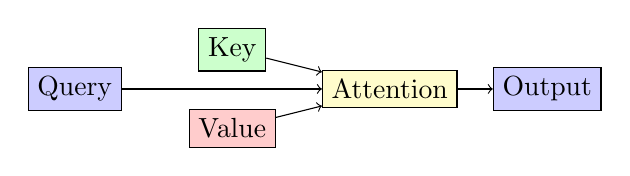
\begin{tikzpicture}
        \node[rectangle, draw, fill=blue!20] (Q) at (0,1) {Query};
        \node[rectangle, draw, fill=green!20] (K) at (2,1.5) {Key};
        \node[rectangle, draw, fill=red!20] (V) at (2,0.5) {Value};
        \node[rectangle, draw, fill=yellow!20] (A) at (4,1) {Attention};
        \node[rectangle, draw, fill=blue!20] (O) at (6,1) {Output};
        \draw[->] (Q) -- (A);
        \draw[->] (K) -- (A);
        \draw[->] (V) -- (A);
        \draw[->] (A) -- (O);
    \end{tikzpicture}
    \caption{Attention mechanism in neural networks.}
    \label{fig:attention}
\end{figure}
